% background chapter continued
\section{Mercator Architecture}\label{blueprint}
This section proceeds into detailed description of Mercator\cite{mercator} web crawler surveyed in section \ref{relatedworks}. Figure \ref{fig:basicarch} is a high-level composition of the same. As seen, Mercator specializes different steps defined in basic crawling
algorithm covered in section \ref{basicalgo} and adds several other steps to address
the social and scalability challenges of web crawler. Its blueprint design offers
horizontal scalability and therefore if implemented can run on more than one node.
Each part that contributes to mercator crawler can also be referred to as a
component, module, subsystem, etc. They can be used interchangeably from this point onward.

\begin{figure}[h!]
  \centering
  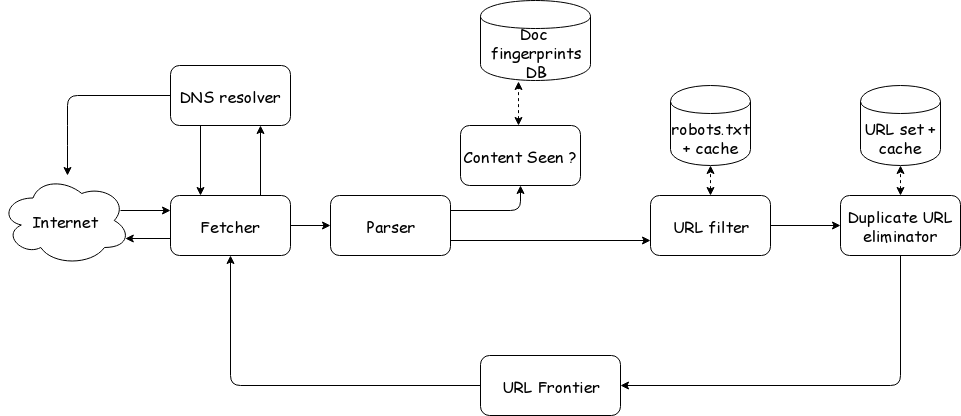
\includegraphics[width=15cm,height=12cm,keepaspectratio]{../media/crawler/basic-crawler-architecture-v2.png}
  \caption{High-level organization of Mercator}
  \label{fig:basicarch}
\end{figure}

\noindent
Each work cycle begins and ends at the URL Frontier. Depending on what needs to be
achieved, the entire crawler can run as a single process or can be partitioned into multiple processes - treating each subsystem as a process. Given a single URL, it
goes through the cycle of being fetched followed by passing through various checks,
filters and eliminations, then finally returned to the Frontier (for incremental crawling).
\\
\\
At the beginning of each logical loop cycle, a worker thread pops a URL from the Frontier data structure adhering to the priority and politeness policy. The output URL is then fetched by HTTP fetcher subsystem - which like any other web client contacts DNS module to get IP address of the corresponding web server. The web page is then retrieved and stored at a temporary location which is then picked up by parser subsystem which forwards the path to the page and extracted links to content seen and URL filter, respectively. The batch of URLs undergo a fixed set of pre-processing steps at the URL filter subsystem before being passed over to Duplicate URL eliminator (DUE). The DUE module tests each URL to determine whether the link should be added to the
URL frontier.

\pagebreak

\subsection{Fetcher, Parser, and DNS}\index{Fetcher, Parser, and DNS}
It occurred to designers of Mercator that the task of fetching each URL from seed set or newly discovered
links is complex. First, the request made to the web server at a given URL endpoint will have several outcomes as a response. Therefore, it becomes a bottleneck to implemented fetcher as only single threaded, blocking synchronous module. Instead it should be written as a multi-threaded, synchronous I/O or non-block,
asychronous I/O to speedup the operation. Moreover, it is also inefficient to have DNS resolve a given URL's
IP address each time a fetch request is made to the same web server. This can be fixed by having a cache of
lookup pair for each web host in the frontier. According to Mercator designers, another difficulty is the lookup implementation itself of DNS entries is blocking; meaning that at a time only one request is considered and completed and all other requests queue up. The solution for this is yet again a multi-threaded approach
or a asynchronous I/O wrapper.

\subsection{Handling De-duplication}\index{Handling De-duplication}
Any professional or sophisticated crawler has the capability to minimize De-duplication. De-duplication
simply tests whether a web page with the same content has already been seen at another URL. As per
figure \ref{fig:basicarch}, the content seen subsystem takes care of the same. There exist three
established methods to solve this problem. 

\begin{enumerate}
  \item Document fingerprinting (checksums)
  \item Bloom Filters
  \item Shingles
\end{enumerate}

(\textit{this will be expanded further})

\pagebreak

\subsection{URL Filtering}\index{URL Filtering}
The URL Filter component takes input a batch of extracted URLs, applies a series of tests, modifiers on each URL, composes a newer batch of URL which fall in its
criteria and forwards it to the next subsystem. For instance, assume a set of links $\sum_{n=1}^{10}$ $ U_n$ extracted from page $p$, there is a possibility that some $U$'s link are relative to the page $p$, in
such cases, this component normalizes such $U$'s turning them into absolute URLs. Also, the crawler can
enforce a rule to exclude out of bound URls - those that don't fall within a given list of domains. 

\begin{figure}[h!]
  \centering
  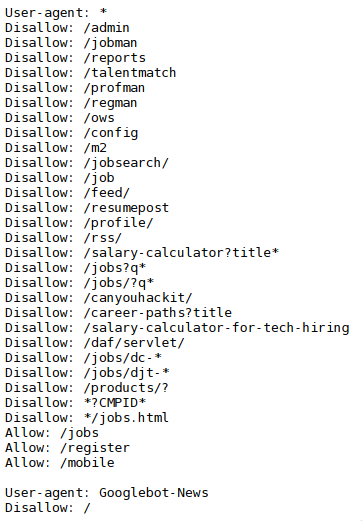
\includegraphics[width=8cm,height=13cm,keepaspectratio]{../media/crawler/robots-txt-sample.png}
  \caption{Robots Exclusion Policy set by dice.com}
  \label{fig:robotsdice}
\end{figure}

\noindent
Apart from these, many hosts regulate whats allowed/not-allowed for downloading by placing a \textit{robots.txt} file under root directory of a hosted web site. The standard is known as Robot Exclusion Protocol.
Figure \ref{fig:robotsdice} shows a \textit{robots.txt} of dice.com. Its interpretation beginning at line one goes like no crawler should visit \textit{/admin}, \textit{/jobman} pages, but it can visit \textit{/jobs},
\textit{/register}, and so on. A user-agent containing string Googlebot-news is not legally allowed to
crawl  any of its pages. For each domain, the crawler fetches robots.txt to test whether the URL under consideration passes the robot restrictions and only then it is added to its Frontier data structure. Given a
high locality that many of the extracted links fall within the domain, it is efficient to cache robots.txt rule into an in-memory data store. The cache expires and redownloads robots.txt for each domain several times a day to stay in sync with the rule changes.
\\
\\
It should be noted that it is always safer and courteous to include a note in request header of the crawler indicating intentions to download the data, and also provide your email address where the webmaster can contact you in case of any issues. Also, it is a good practice to enforce strict compliance with domain's robots.txt rules.

\subsection{Duplicate URL Eliminator (DUE)}\index{Duplicate URL Eliminator(DUE)}
A batch of URLs qualified from URL filtering subsystem arrives at DUE. Sometimes it s also referred to URL-seen test. DUE guards the URL Frontier by eliminating
multiple instances of the same URL from adding to the Frontier. It also keeps history of set of URLs that were previously added to the URL Frontier and those that are
currently in it. The fire-and-forget, one-time crawl URLs are only crawled once. In
continuous crawling Frontier scheme, some URLs are revisited periodically for new information, in such cases, the DUE has to delete its traces from its state.
\\
\\
\noindent
Understanding the behavior of DUE explained in above paragraph, the size of URL set stored in relational database on disk will grow linearly as the size of web corpus grows irrespective of whether the crawler is continuous/non-continuous. Since the DUE has to make sure that it isn't adding duplicate URL to the Frontier, it will check against each entry in the URL set table. This will hamper DUE throughput and increase disk seek latency over time i.e the time taken to check and respond for existing entry increases. Each insertion in the URL set table is a fixed size checksum of
textual URL along with the mapping to URL itself. The checksum algorithm should be
such that it has exponentially small probabilistic bounds on the likelihood of
collision in the URL set.
\\
\\
To reduce the number of operations required to DUE each URL in a batch, several
optimizations can be combined. First, keeping an in-memory cache objects of popular URLs. The intuition for this is continuous crawling URLs endpoint will be revisited. But again with this, the cache hit rate is low as ratio of continuous to one-time crawls can be 20:1. Also as the computed checksums of the URLs are highly unique, it has lower locality, so the checksums that miss the cache will require disk access and disk seek. Secondly, taking advantage of high locality of checksum hostname(domain name) concatenating with checksum of absolute URL for that domain name results in
same host names being numerically closer to each other. This in turn translates to
access locality on the URL set.

\pagebreak

\subsection{URL Frontier}
some text here
\begin{figure}[h!]
  \centering
  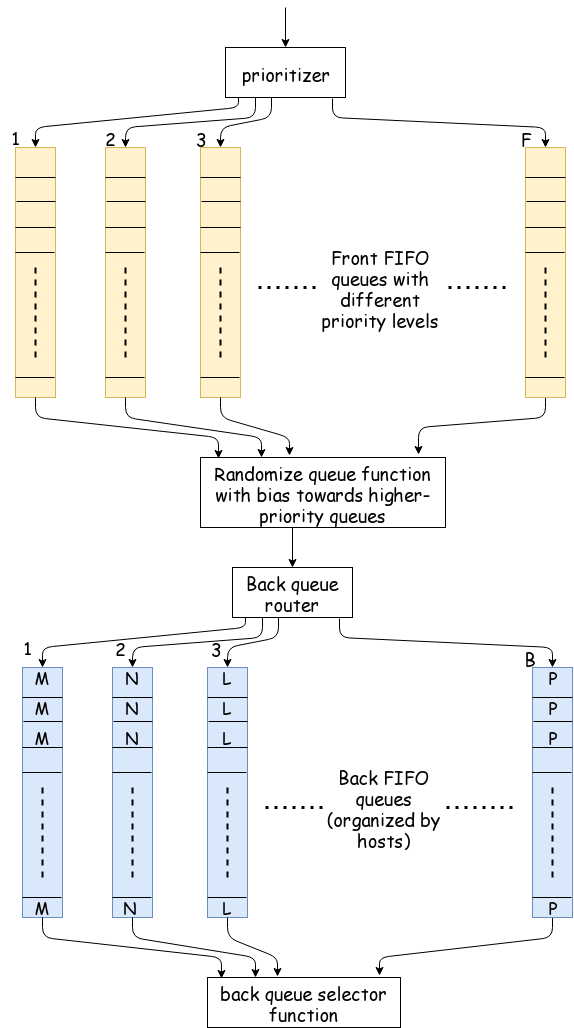
\includegraphics[width=10cm,height=13cm,keepaspectratio]{../media/crawler/url-frontier.png}
  \caption{URL Frontier Scheme(based on Mercator)}
  \label{fig:frontier}
\end{figure}

\pagebreak
some text here
\begin{figure}[h!]
  \centering
  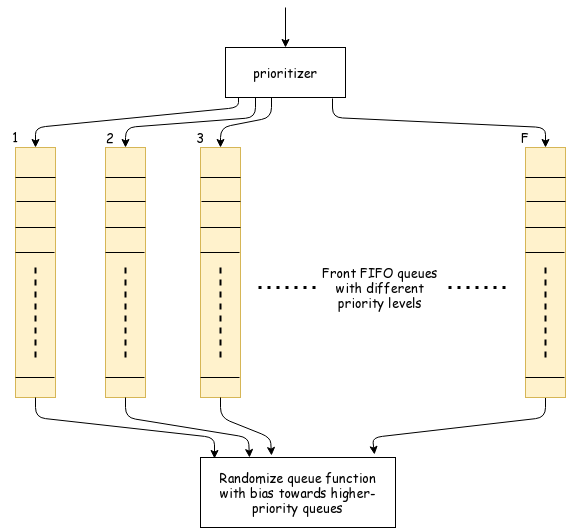
\includegraphics[width=13cm,height=10cm,keepaspectratio]{../media/crawler/f-queue.png}
  \caption{Frontier Front Queue}
  \label{fig:fqueue}
\end{figure}

\pagebreak
some text here
\begin{figure}[h!]
  \centering
  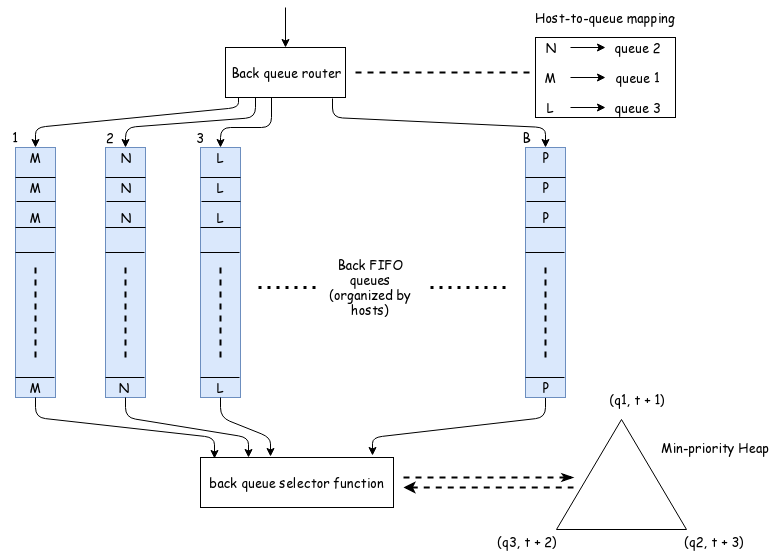
\includegraphics[width=13cm,height=10cm,keepaspectratio]{../media/crawler/b-queue.png}
  \caption{Frontier Back Queue}
  \label{fig:bqueue}
\end{figure}

\pagebreak
some text here
\subsection{Distributing Web Crawl}\index{Distributing Web Crawl}
\begin{figure}[h!]
  \centering
  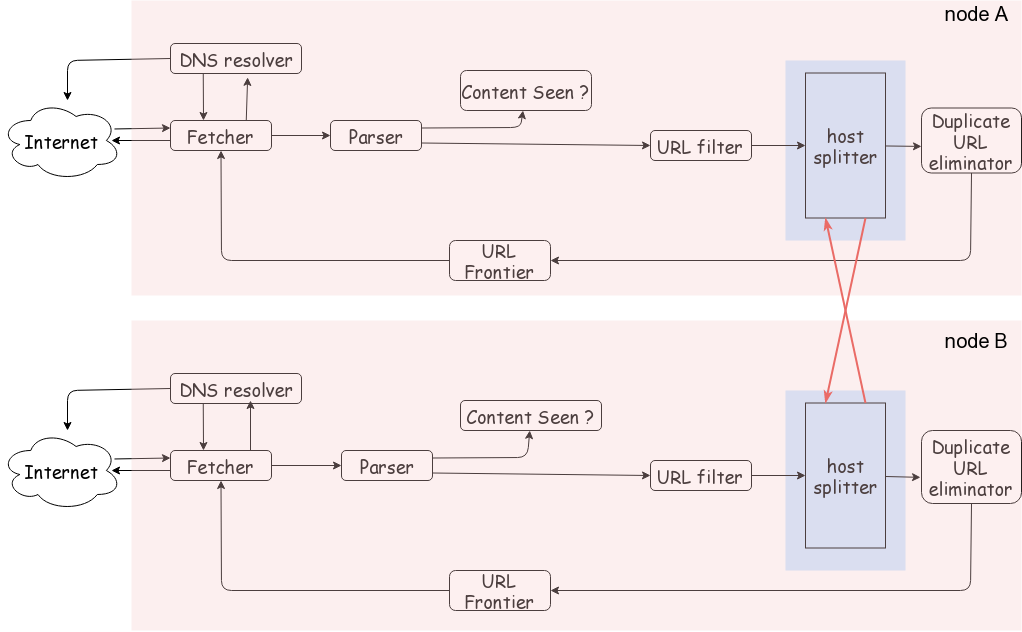
\includegraphics[width=15cm,height=10cm,keepaspectratio]{../media/crawler/host-splitterv3.png}
  \caption{Host Partitioning}
  \label{fig:hpart}
\end{figure}

\pagebreak

\section{Automata Analogy}\index{Automata Analogy}